\documentclass[aspectratio=169,10pt]{beamer}
\usetheme{Madrid}
\usecolortheme{dolphin}
\usefonttheme{professionalfonts}
\usepackage[T1]{fontenc}
\usepackage{lmodern}
\usepackage{amsmath,amssymb,mathtools}
\usepackage{booktabs,array}
\usepackage{tikz}
\usetikzlibrary{arrows.meta,positioning,calc}

\definecolor{DLSblue}{HTML}{12355B}
\definecolor{DLScyan}{HTML}{168AAD}
\definecolor{DLSgold}{HTML}{F2A541}
\definecolor{DLSlight}{HTML}{EEF6F8}
\setbeamercolor{structure}{fg=DLSblue}
\setbeamercolor{frametitle}{bg=DLSblue,fg=white}
\setbeamercolor{block title}{bg=DLScyan,fg=white}
\setbeamercolor{block body}{bg=DLSlight,fg=black}
\setbeamertemplate{navigation symbols}{}
\setbeamertemplate{footline}{%
  \leavevmode\hbox{%
  \begin{beamercolorbox}[wd=.82\paperwidth,ht=2.5ex,dp=1ex,leftskip=1em]{author in head/foot}
    Deep Learning Systems 2026 \hfill Einsum Architectures
  \end{beamercolorbox}%
  \begin{beamercolorbox}[wd=.18\paperwidth,ht=2.5ex,dp=1ex,center]{date in head/foot}
    \insertframenumber/\inserttotalframenumber
  \end{beamercolorbox}}}
\newcommand{\shape}[1]{\textcolor{DLScyan}{\ensuremath{#1}}}
\newcommand{\idx}[1]{\textcolor{DLSgold!80!black}{\ensuremath{#1}}}
\newcommand{\einsum}[1]{\texttt{#1}}
\newcommand{\key}[1]{\textbf{\textcolor{DLSblue}{#1}}}
\newcommand{\codebox}[1]{\begin{beamercolorbox}[rounded=true,sep=0.7ex]{block body}\ttfamily #1\end{beamercolorbox}}

\title{Einstein Summation as an Architecture Language}
\subtitle{MLPs, CNNs, GNNs, LSTMs, and Transformers in \texttt{torch.einsum}}
\author{DeepLearningSystems-2026}
\institute{From index equations to efficient kernels}
\date{2026}

\begin{document}

% 1
\begin{frame}[plain]
  \titlepage
  \vfill
  \centering\small One notation for expressing computation, checking shapes, and reasoning about systems costs.
\end{frame}

% 2
\begin{frame}{Learning objectives and route}
\begin{columns}[T]
\column{0.48\textwidth}
By the end, you can:
\begin{itemize}
  \item read free and contracted indices;
  \item translate equations into \texttt{torch.einsum};
  \item derive five common architectures;
  \item predict FLOPs, intermediates, and fusion opportunities;
  \item test an expression with explicit shapes.
\end{itemize}
\column{0.48\textwidth}
\centering
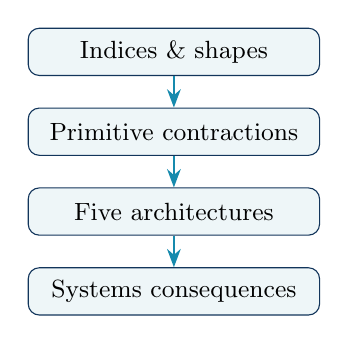
\begin{tikzpicture}[node distance=4mm, every node/.style={font=\small}, box/.style={draw=DLSblue,rounded corners,fill=DLSlight,minimum width=3.7cm,minimum height=6mm},arr/.style={-{Stealth},thick,DLScyan}]
\node[box] (n) {Indices \& shapes};
\node[box,below=of n] (p) {Primitive contractions};
\node[box,below=of p] (a) {Five architectures};
\node[box,below=of a] (s) {Systems consequences};
\draw[arr] (n)--(p); \draw[arr] (p)--(a); \draw[arr] (a)--(s);
\end{tikzpicture}
\end{columns}
\end{frame}

% 3
\begin{frame}{Einstein notation: indices carry the specification}
\[
  C_{ij}=\sum_k A_{ik}B_{kj}
\]
\begin{columns}[T]
\column{0.50\textwidth}
\begin{block}{Two roles}
\begin{itemize}
 \item \key{Free indices} $i,j$ survive in the output.
 \item \key{Contracted index} $k$ appears in inputs but not output, so it is summed.
\end{itemize}
\end{block}
\column{0.46\textwidth}
\begin{block}{Shape contract}
$A:\shape{[I,K]}$, $B:\shape{[K,J]}$, $C:\shape{[I,J]}$.

Repeated labels must have compatible extent. Output label order fixes output axis order.
\end{block}
\end{columns}
\vspace{0.4em}
\codebox{torch.einsum('ik,kj->ij', A, B)}
\end{frame}

% 4
\begin{frame}{From nested loops to one contraction}
\begin{columns}[T]
\column{0.48\textwidth}
\begin{block}{Literal algorithm}
\ttfamily\small
for i in range(I):\\
\quad for j in range(J):\\
\qquad C[i,j] = 0\\
\qquad for k in range(K):\\
\qquad\quad C[i,j] += A[i,k]*B[k,j]
\end{block}
\column{0.48\textwidth}
\begin{block}{Declarative algorithm}
\[
\einsum{ik,kj->ij}
\]
The labels state:
\begin{itemize}
 \item iteration space: $i,j,k$;
 \item reduction: $k$;
 \item output layout: $i,j$.
\end{itemize}
\end{block}
\end{columns}
\begin{alertblock}{Important}
Einsum specifies the result, not a unique loop order or kernel. The implementation still chooses tiling, fusion, and contraction order.
\end{alertblock}
\end{frame}

% 5
\begin{frame}{The einsum grammar: keep, sum, broadcast, diagonalize}
\small
\begin{tabular}{lll}
\toprule
Operation & Equation / subscript & Output shape \\
\midrule
Dot product & $x_i y_i$ / \einsum{`i,i->'} & scalar \\
Outer product & $x_i y_j$ / \einsum{`i,j->ij'} & $[I,J]$ \\
Batch matmul & $A_{bik}B_{bkj}$ / \einsum{`bik,bkj->bij'} & $[B,I,J]$ \\
Broadcast weights & $X_{bti}W_{io}$ / \einsum{`bti,io->bto'} & $[B,T,O]$ \\
Trace & $A_{ii}$ / \einsum{`ii->'} & scalar \\
Diagonal & $A_{ii}$ / \einsum{`ii->i'} & $[I]$ \\
\bottomrule
\end{tabular}
\vspace{0.8em}
\begin{block}{Rule of thumb}
A label repeated within one operand selects a diagonal. A label absent after \texttt{->} is reduced. Ellipsis \texttt{...} denotes unnamed broadcast dimensions.
\end{block}
\end{frame}

% 6
\begin{frame}{Shape discipline: a four-step correctness test}
\begin{enumerate}
 \item \key{Name every axis}: e.g., batch $b$, token $t$, feature $d$.
 \item \key{Write operand shapes}: $X:[B,T,D]$, $W:[D,O]$.
 \item \key{Check each shared label}: every $d$ must mean the same extent $D$.
 \item \key{Read output labels}: \einsum{btd,do->bto} gives $[B,T,O]$.
\end{enumerate}
\begin{exampleblock}{Executable shape assertion}
\ttfamily\small
B,T,D,O = 2,7,16,32\\
x = torch.randn(B,T,D); w = torch.randn(D,O)\\
y = torch.einsum('btd,do->bto', x, w)\\
assert y.shape == (B,T,O)
\end{exampleblock}
\begin{alertblock}{Frequent bug}
Reusing a letter for different semantic axes may silently compute the wrong result when the extents happen to match.
\end{alertblock}
\end{frame}

% 7
\begin{frame}{MLP: an affine layer is a batched contraction}
For $X:\shape{[B,I]}$, $W:\shape{[I,O]}$, $a:\shape{[O]}$:
\[
 Z_{bo}=\sum_i X_{bi}W_{io}+a_o, \qquad H_{bo}=\phi(Z_{bo}).
\]
\codebox{Z = torch.einsum('bi,io->bo', X, W) + a}
\vspace{0.5em}
\begin{columns}[T]
\column{0.48\textwidth}
\begin{block}{What einsum covers}
The dense linear map and any leading batch-like axes.
\end{block}
\column{0.48\textwidth}
\begin{block}{What it does not cover}
Bias addition and nonlinear activation are elementwise operations, often fused by a compiler.
\end{block}
\end{columns}
\begin{exampleblock}{Cost}
Approximately $2BIO$ floating-point operations; weights contribute $IO$ parameters.
\end{exampleblock}
\end{frame}

% 8
\begin{frame}{MLP over tokens and stacked experts}
\small
\begin{block}{Token-wise projection}
$X:[B,T,D]$, $W:[D,F]$:
\[
H_{btf}=\sum_d X_{btd}W_{df},\qquad
\einsum{btd,df->btf}.
\]
Weights are reused independently at every $b,t$.
\end{block}
\begin{block}{Expert-specific projection}
$W:[E,D,F]$ gives $H_{btef}=\sum_d X_{btd}W_{edf}$, or
\einsum{btd,edf->btef}. This materializes all expert outputs.
\end{block}
\begin{alertblock}{Systems question}
Materialize $[B,T,E,F]$, or gather routed tokens and issue grouped matrix multiplies?
\end{alertblock}
\end{frame}

% 9
\begin{frame}{CNN: expose patches, then contract}
Let patches $P:\shape{[B,H_o,W_o,C_i,K_h,K_w]}$ and kernels $K:\shape{[C_o,C_i,K_h,K_w]}$.
\[
Y_{bhw o}=\sum_{cuv}P_{bhwcuv}K_{ocuv}
\]
\codebox{Y = torch.einsum('bhwcuv,ocuv->bhwo', P, K)}
\begin{columns}[T]
\column{0.48\textwidth}
\begin{block}{Index meaning}
$b$: batch; $h,w$: output location; $c$: input channel; $u,v$: kernel offset; $o$: output channel.
\end{block}
\column{0.48\textwidth}
\begin{block}{Equivalent view}
Flatten $(c,u,v)$ into one reduction axis. Convolution becomes a matrix multiplication after \emph{im2col}.
\end{block}
\end{columns}
\end{frame}

% 10
\begin{frame}{CNN systems view: arithmetic versus movement}
\begin{columns}[T]
\column{0.49\textwidth}
\begin{block}{Explicit patches}
\begin{itemize}
 \item Simple GEMM lowering.
 \item Patch tensor size: $BH_oW_oC_iK_hK_w$.
 \item Repeats overlapping input pixels.
\end{itemize}
\end{block}
\column{0.47\textwidth}
\begin{block}{Implicit / direct convolution}
\begin{itemize}
 \item Generate patch addresses on demand.
 \item Tile input and kernels in fast memory.
 \item Avoid full im2col materialization.
\end{itemize}
\end{block}
\end{columns}
\begin{exampleblock}{Compute count}
$\approx 2BH_oW_oC_oC_iK_hK_w$ FLOPs. Performance depends on reuse and layout, not only this count.
\end{exampleblock}
\begin{alertblock}{Mini-check}
If $K_h=K_w=1$, which indices disappear? The operation reduces to a per-pixel channel projection: \einsum{bhwc,oc->bhwo}.
\end{alertblock}
\end{frame}

% 11
\begin{frame}{GNN: neighborhood aggregation as a contraction}
For dense adjacency $A:\shape{[N,N]}$ and node features $X:\shape{[N,D]}$:
\[
M_{id}=\sum_j \widehat{A}_{ij}X_{jd},
\qquad \einsum{ij,jd->id}.
\]
Then apply a learned projection $W:\shape{[D,F]}$:
\[
H_{if}=\sum_d M_{id}W_{df},
\qquad \einsum{id,df->if}.
\]
\begin{block}{Combined equation}
\[
H_{if}=\sum_{j,d}\widehat{A}_{ij}X_{jd}W_{df},
\qquad \einsum{ij,jd,df->if}.
\]
\end{block}
\begin{alertblock}{Reality check}
Real graphs are sparse: use scatter/segment reductions or sparse matrix multiply, not dense $N\times N$ adjacency.
\end{alertblock}
\end{frame}

% 12
\begin{frame}{GNN layer: semantics and execution}
\begin{columns}[T]
\column{0.48\textwidth}
\centering
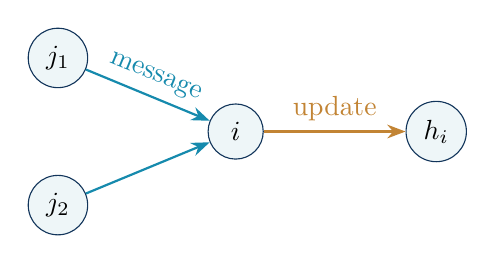
\begin{tikzpicture}[>=Stealth,node distance=11mm,vertex/.style={circle,draw=DLSblue,fill=DLSlight,minimum size=7mm}, every edge/.style={draw=DLScyan,thick,->}]
\node[vertex] (j1) {$j_1$};
\node[vertex,below=of j1] (j2) {$j_2$};
\node[vertex,right=19mm of $(j1)!0.5!(j2)$] (i) {$i$};
\node[vertex,right=18mm of i] (h) {$h_i$};
\draw[->,thick,DLScyan] (j1)--node[above,sloped]{message}(i);
\draw[->,thick,DLScyan] (j2)--(i);
\draw[->,thick,DLSgold!80!black] (i)--node[above]{update}(h);
\end{tikzpicture}
\column{0.48\textwidth}
\begin{enumerate}
 \item Gather source features $X_j$.
 \item Form edge messages.
 \item Reduce messages by destination $i$.
 \item Apply projection / nonlinearity.
\end{enumerate}
\end{columns}
\begin{block}{Contraction-order choice}
$(\widehat A X)W$ costs aggregation in width $D$; $\widehat A(XW)$ costs aggregation in width $F$. Choose based on $D$, $F$, sparsity, and reuse. Associativity preserves the linear result.
\end{block}
\end{frame}

% 13
\begin{frame}{LSTM: fuse four gate projections}
At time $t$, concatenate input and previous hidden state conceptually:
\[
G_{brg}=\sum_d S_{bd}W_{drg}+a_{rg},
\quad S=[x_t;h_{t-1}],\quad r\in\{i,f,o,g\}.
\]
Shapes: $S:\shape{[B,D]}$, $W:\shape{[D,4,H]}$, $G:\shape{[B,4,H]}$.
\codebox{G = torch.einsum('bd,drh->brh', S, W) + a}
\begin{block}{Why fuse?}
One larger matrix multiplication reuses $S$, reduces launch overhead, and usually outperforms four separate projections.
\end{block}
\begin{alertblock}{Notation warning}
Here $r$ is the gate axis and $h$ is the hidden-feature axis; do not reuse $h$ for the hidden-state tensor name inside the index equation.
\end{alertblock}
\end{frame}

% 14
\begin{frame}{LSTM recurrence: contraction plus elementwise state update}
Split $G$ along its gate axis and apply nonlinearities:
\[
 i_t=\sigma(G_i),\quad f_t=\sigma(G_f),\quad
 o_t=\sigma(G_o),\quad \widetilde c_t=\tanh(G_g).
\]
\[
 c_t=f_t\odot c_{t-1}+i_t\odot\widetilde c_t,
 \qquad h_t=o_t\odot\tanh(c_t).
\]
\begin{columns}[T]
\column{0.48\textwidth}
\begin{block}{Parallel within a step}
All four affine gate computations are one contraction.
\end{block}
\column{0.48\textwidth}
\begin{block}{Sequential across time}
$(h_t,c_t)$ depends on $(h_{t-1},c_{t-1})$; sequence steps form a critical path.
\end{block}
\end{columns}
\begin{exampleblock}{Systems implication}
Kernel fusion helps inside each step, but recurrence limits time-axis parallelism; scan methods trade extra work for parallel depth.
\end{exampleblock}
\end{frame}

% 15
\begin{frame}{Transformer I: project tokens into heads}
Input $X:\shape{[B,T,D]}$; projection weights $W^Q,W^K,W^V:\shape{[D,H,P]}$.
\[
Q_{bthp}=\sum_d X_{btd}W^Q_{dhp}
\]
\codebox{Q = torch.einsum('btd,dhp->bthp', X, Wq)}
\vspace{0.35em}
Analogously obtain $K,V:\shape{[B,T,H,P]}$. Often the three weights are packed:
\[
R_{btzhp}=\sum_d X_{btd}W_{zdhp},\qquad z\in\{Q,K,V\}.
\]
\codebox{R = torch.einsum('btd,zdhp->btzhp', X, Wqkv)}
\begin{block}{Implementation note}
Production kernels commonly flatten $(H,P)$ and use GEMM; the explicit head labels remain valuable for reasoning and tests.
\end{block}
\end{frame}

% 16
\begin{frame}{Transformer II: attention scores and weighted values}
\begin{columns}[T]
\column{0.54\textwidth}
\[
S_{bhts}=\frac{1}{\sqrt P}\sum_p Q_{bthp}K_{bshp}
\]
\codebox{S = torch.einsum('bthp,bshp->bhts', Q, K) / sqrt(P)}
\[
A=\operatorname{softmax}_s(S+M),\qquad
O_{bthp}=\sum_s A_{bhts}V_{bshp}.
\]
\codebox{O = torch.einsum('bhts,bshp->bthp', A, V)}
\column{0.42\textwidth}
\centering
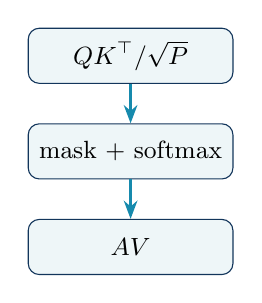
\begin{tikzpicture}[node distance=5mm,box/.style={draw=DLSblue,rounded corners,fill=DLSlight,minimum width=2.6cm,minimum height=7mm,font=\small},arr/.style={-{Stealth},thick,DLScyan}]
\node[box] (qk) {$QK^\top/\sqrt P$};
\node[box,below=of qk] (m) {mask + softmax};
\node[box,below=of m] (av) {$AV$};
\draw[arr](qk)--(m);\draw[arr](m)--(av);
\end{tikzpicture}
\end{columns}
\end{frame}

% 17
\begin{frame}{Transformer III: merge heads and project}
Attention output $O:\shape{[B,T,H,P]}$ and output weight $W^O:\shape{[H,P,D]}$:
\[
Y_{btd}=\sum_{h,p}O_{bthp}W^O_{hpd}.
\]
\codebox{Y = torch.einsum('bthp,hpd->btd', O, Wo)}
\begin{block}{Full attention tensor shapes}
\centering
\begin{tabular}{ccccc}
$X$ & $Q,K,V$ & $S,A$ & $O$ & $Y$ \\
$[B,T,D]$ & $[B,T,H,P]$ & $[B,H,T,T]$ & $[B,T,H,P]$ & $[B,T,D]$
\end{tabular}
\end{block}
\begin{alertblock}{Memory bottleneck}
Materializing $A$ costs $O(BHT^2)$ elements. FlashAttention tiles the score computation and online softmax so the full matrix need not reside in high-bandwidth memory.
\end{alertblock}
\end{frame}

% 18
\begin{frame}{Systems lens: equivalent equations, unequal executions}
\small
\begin{tabular}{p{0.22\textwidth}p{0.30\textwidth}p{0.38\textwidth}}
\toprule
Decision & Question & Typical response \\
\midrule
Contraction order & Which intermediate is smallest? & Reassociate linear contractions; use an optimizer for $\ge3$ operands.\\
Layout & Are reduction axes contiguous? & Permute/pack once, then feed GEMM-friendly tiles.\\
Materialization & Is an intermediate reused enough? & Fuse producer--consumer or recompute cheap values.\\
Sparsity & Are most coefficients zero? & Store edges/blocks; use segmented or sparse kernels.\\
Precision & What range/accuracy is required? & Low-precision inputs, wider accumulation, scaling.\\
Batching & Are shapes regular? & Pad/bucket, grouped GEMM, or shape-specialized kernels.\\
\bottomrule
\end{tabular}
\vspace{0.5em}
\begin{block}{Roofline reminder}
Speed is bounded by $\min(\text{peak FLOP/s},\ \text{bandwidth}\times\text{arithmetic intensity})$. Einsum reveals reuse opportunities but does not guarantee they are realized.
\end{block}
\end{frame}

% 19
\begin{frame}{Mini-exercises: predict before you run}
\small
\begin{enumerate}
 \item $X:[8,128,64]$, $W:[64,256]$. Write the token-wise projection and output shape.
 \item For \einsum{bik,bkj->bij}, which index is reduced? What are the compatibility constraints?
 \item Rewrite a $1\times1$ convolution for NHWC input as an einsum.
 \item In dense GNN propagation, compare $(AX)W$ with $A(XW)$ when $D=1024$ and $F=64$.
 \item For attention with $B=4,H=8,T=2048$, how many elements are in the score tensor?
\end{enumerate}
\begin{exampleblock}{Answers}
\begin{enumerate}
 \item \einsum{btd,df->btf}, shape $[8,128,256]$.
 \item $k$; batch $b$ and contracted extent $k$ must agree.
 \item \einsum{bhwc,oc->bhwo}.
 \item Project first to aggregate 64-wide features, subject to sparsity/kernel details.
 \item $4\cdot8\cdot2048^2=134{,}217{,}728$ elements (about 256 MiB in FP16).
\end{enumerate}
\end{exampleblock}
\end{frame}

% 20
\begin{frame}{Takeaways and references}
\begin{columns}[T]
\column{0.52\textwidth}
\begin{block}{Five durable habits}
\begin{enumerate}
 \item Name axes by meaning.
 \item Distinguish free from reduced indices.
 \item Assert shapes with tiny tensors.
 \item Separate mathematical equivalence from execution cost.
 \item Inspect intermediates, layout, and memory traffic.
\end{enumerate}
\end{block}
\column{0.44\textwidth}
\begin{block}{Further reading}
\footnotesize
\begin{itemize}
 \item PyTorch, \emph{torch.einsum documentation}.
 \item Kolda \& Bader, \emph{Tensor Decompositions and Applications}, 2009.
 \item Vaswani et al., \emph{Attention Is All You Need}, 2017.
 \item Dao et al., \emph{FlashAttention}, 2022.
 \item Hamilton, \emph{Graph Representation Learning}, 2020.
\end{itemize}
\end{block}
\end{columns}
\vfill
\centering\Large\color{DLSblue}\textbf{Indices are a compact architecture specification.}
\end{frame}

\end{document}
